
% This file is part of the Openlab-Template project
% Copyright (c) 2015 Jimmy Aguilar Mena.
% 
% This program is free software: you can redistribute it and/or modify  
% it under the terms of the GNU General Public License as published by  
% the Free Software Foundation, version 3.
%
% This program is distributed in the hope that it will be useful, but 
% WITHOUT ANY WARRANTY; without even the implied warranty of 
% MERCHANTABILITY or FITNESS FOR A PARTICULAR PURPOSE. See the GNU 
% General Public License for more details.
%
% You should have received a copy of the GNU General Public License 
% along with this program. If not, see <http://www.gnu.org/licenses/>.
%
% This is a basic show example for the OLReport package.
% Jimmy Aguilar Mena. August, 2015
% Any bug report, or comment: kratsbinovish@gmail.com



\documentclass[11pt]{report}
\usepackage{OLReport}

\title{This is the title, it can be relatively long, just try.}
\author{Myname Lastname}
\supervisor{First Supervisor\newline Secound Supervisor}

\begin{document}
\maketitle
\begin{specification}
	This are the specifications bla bla bla
\end{specification}

\begin{abstract}
	This is the abstract remember this will not have numbers.
\end{abstract}

\tableofcontents
\newpage

\section{Introduction}
This is my very long introduction This is my very long introduction This is my very long introduction This is my very long introduction This is my very long introduction This is my very long introduction 

\section{This is a new section}
Here the text and the numeration is as usual in the original template the introduction is numerated.

\section{Another seccion}
Another section text

\subsection{My subseccion}
Subsection text

\subsubsection{Now a subsubseccion}
Subsubsection text in third level of numeration. After this level there are not numbers

\begin{figure}[h]
	\centering
	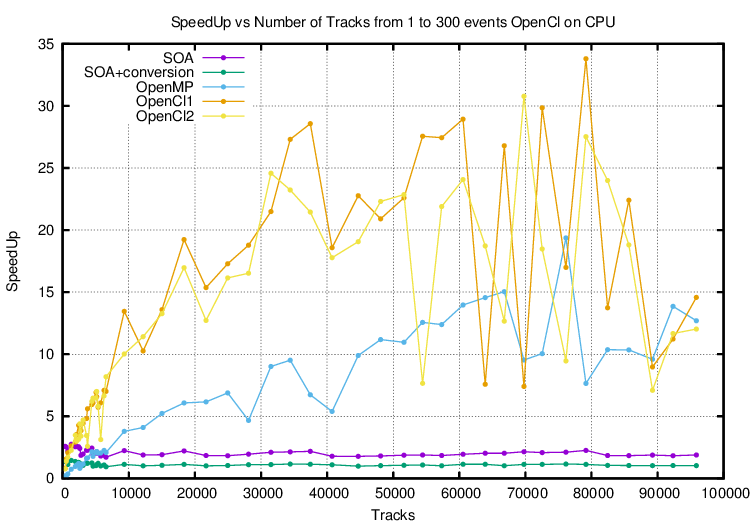
\includegraphics[width=0.7\textwidth]{SU_OMP_Code}
	\caption{This is a figure}
\end{figure}

\begin{table}[h]
	\centering
	\begin{tabular}{|c|c|c|c|c|}
		\hline  &  &  &  &  \\ 
		\hline  &  &  &  &  \\ 
		\hline  &  &  &  &  \\ 
		\hline 
	\end{tabular} 
	\caption{This is a table}
\end{table}


If you add some bibliography use numbered chapter name too. Please complains or problems just inform or solve and contribute :)
\end{document}          
